% Todas las variables de la ELPI 2024 por edad al terremoto.
% Figuras: python3 scripts/37_todo_2024.py
% Compilar desde presentacion/: xelatex todo_2024.tex (dos veces)
\documentclass[aspectratio=169,11pt]{beamer}
\usepackage[spanish,es-nodecimaldot,es-noshorthands]{babel}
\usepackage{fontspec}
\setsansfont{IBMPlexSans}[
  Path=../scripts/fonts/, Extension=.ttf,
  UprightFont=*-Regular, BoldFont=*-SemiBold, ItalicFont=*-Italic]
\usepackage{array}
\usepackage{booktabs}
\usepackage{pifont}

\definecolor{ink}{HTML}{17212B}
\definecolor{acc}{HTML}{2B5FA8}
\definecolor{muted}{HTML}{55606B}
\definecolor{naranja}{HTML}{B4561B}
\definecolor{linea}{HTML}{C9CED3}

\setbeamercolor{normal text}{fg=ink,bg=white}
\setbeamercolor{frametitle}{fg=ink}
\setbeamercolor{structure}{fg=acc}
\setbeamerfont{frametitle}{size=\Large,series=\bfseries}
\setbeamertemplate{navigation symbols}{}
\setbeamertemplate{frametitle}{\vspace*{5mm}\insertframetitle\par}
\setbeamertemplate{footline}{%
  \hfill{\scriptsize\color{muted}\insertframenumber\,/\,\inserttotalframenumber}%
  \hspace*{8mm}\vspace*{4mm}}
\setbeamersize{text margin left=8mm,text margin right=8mm}

\newcommand{\sub}[1]{{\leavevmode\color{muted}#1}}
\newcommand{\nota}[1]{\vfill\noindent\parbox{0.9\textwidth}{\raggedright\scriptsize\color{muted}#1}\par\vspace*{1mm}}
\newcommand{\cita}[1]{{\footnotesize\color{acc}#1}}
\newcommand{\no}{{\leavevmode\color{naranja}\ding{55}}}
\newcommand{\si}{{\leavevmode\color{acc}\ding{51}}}
\newcommand{\canal}[2]{{\leavevmode\bfseries\color{#1}#2}}

\title{Todas las variables de la ELPI 2024}

\begin{document}

\begin{frame}
\frametitle{Todas las variables de la ELPI 2024}
\vspace{2mm}
{\small
\renewcommand{\arraystretch}{1.45}
\begin{tabular}{@{}>{\raggedright\arraybackslash}p{34mm}
                >{\raggedright\arraybackslash}p{104mm}@{}}
\textbf{Qué entra} & Las 571 variables utilizables de las tres bases de 2024:
  adolescente, responsable principal y evaluaciones. Las nominales se separan
  en categorías: 744 resultados en total \\
\textbf{Qué se estima} & Diferencia con quienes tenían 2 años, zona afectada
  menos no afectada, con la especificación del PHQ-4 \\
\textbf{Con p < 0,05} & 5,9 \% a los 6--11 meses, 7,0 \% al año y 6,5 \% a los
  3--4 años; el azar daría el 5 \% \\
\textbf{Color} & Estadístico t, en la codificación de cada variable: azul, más
  bajo; naranja, más alto. No indica si es mejor o peor. * p < 0,10;
  ** p < 0,05; *** p < 0,01 \\
\end{tabular}}

\nota{No entran identificadores, factores de expansión, fechas, códigos
geográficos, texto abierto ni el sexo y la edad del adolescente. De la base del
responsable principal entran las variables del hogar y, de las de cada
integrante, las del adolescente y las del cuidador principal.}
\end{frame}

\begin{frame}
\frametitle{Todas las variables de 2024 (1/10)}
\centering
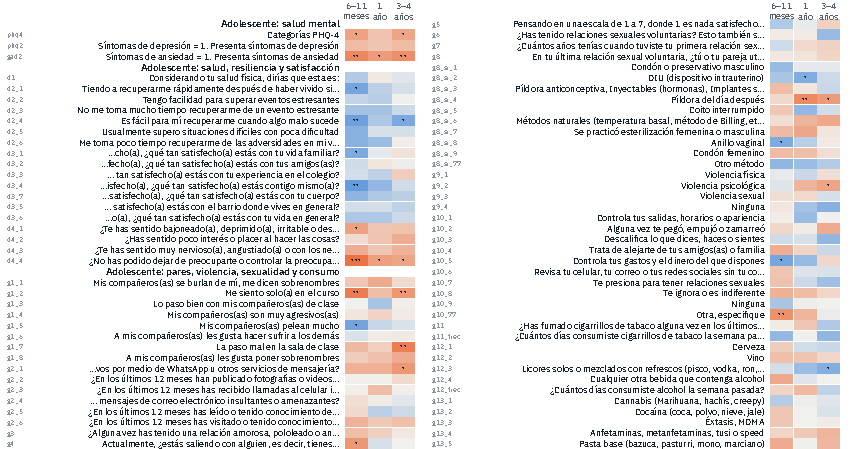
\includegraphics[height=0.83\textheight]{figuras/todo_2024_01.pdf}
\end{frame}
\begin{frame}
\frametitle{Todas las variables de 2024 (2/10)}
\centering
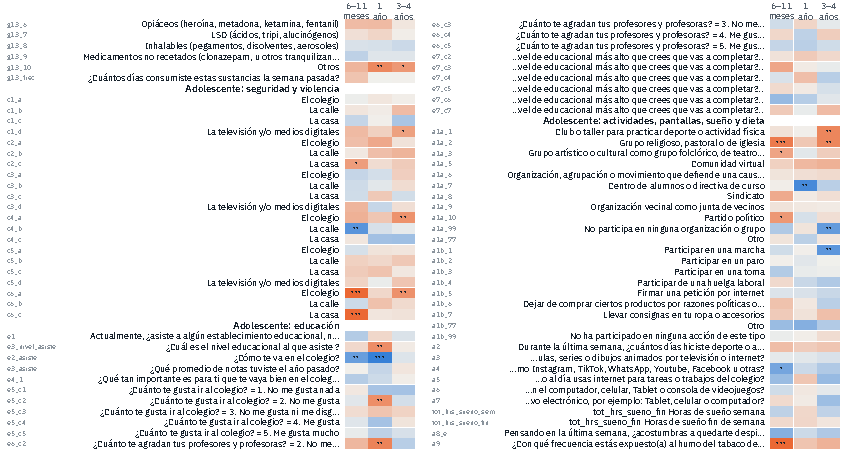
\includegraphics[height=0.83\textheight]{figuras/todo_2024_02.pdf}
\end{frame}
\begin{frame}
\frametitle{Todas las variables de 2024 (3/10)}
\centering
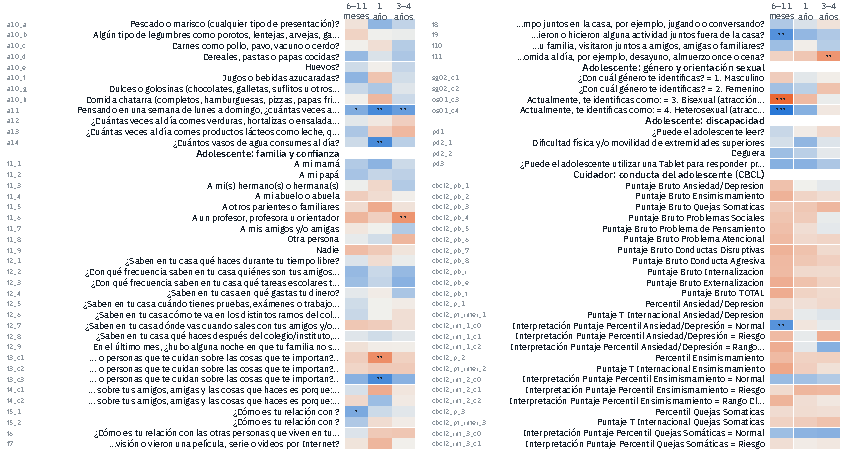
\includegraphics[height=0.83\textheight]{figuras/todo_2024_03.pdf}
\end{frame}
\begin{frame}
\frametitle{Todas las variables de 2024 (4/10)}
\centering
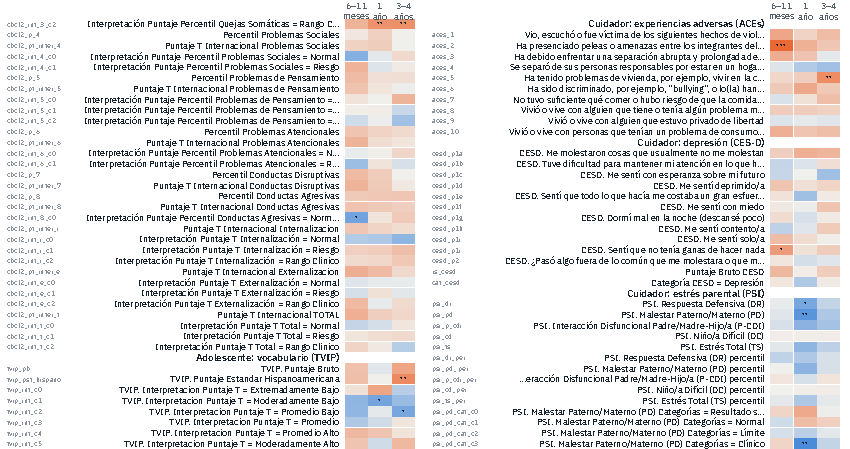
\includegraphics[height=0.83\textheight]{figuras/todo_2024_04.pdf}
\end{frame}
\begin{frame}
\frametitle{Todas las variables de 2024 (5/10)}
\centering
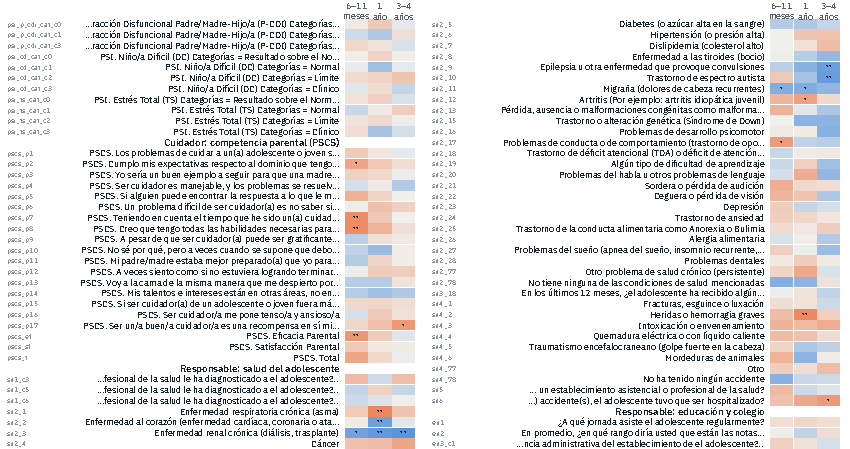
\includegraphics[height=0.83\textheight]{figuras/todo_2024_05.pdf}
\end{frame}
\begin{frame}
\frametitle{Todas las variables de 2024 (6/10)}
\centering
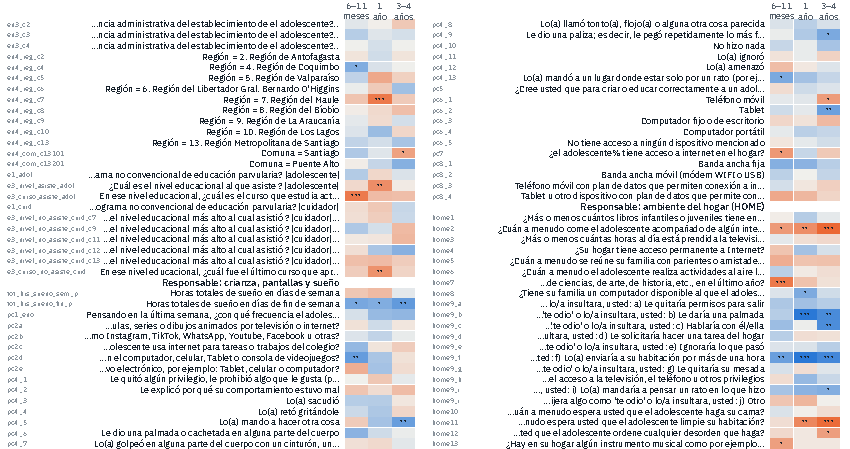
\includegraphics[height=0.83\textheight]{figuras/todo_2024_06.pdf}
\end{frame}
\begin{frame}
\frametitle{Todas las variables de 2024 (7/10)}
\centering
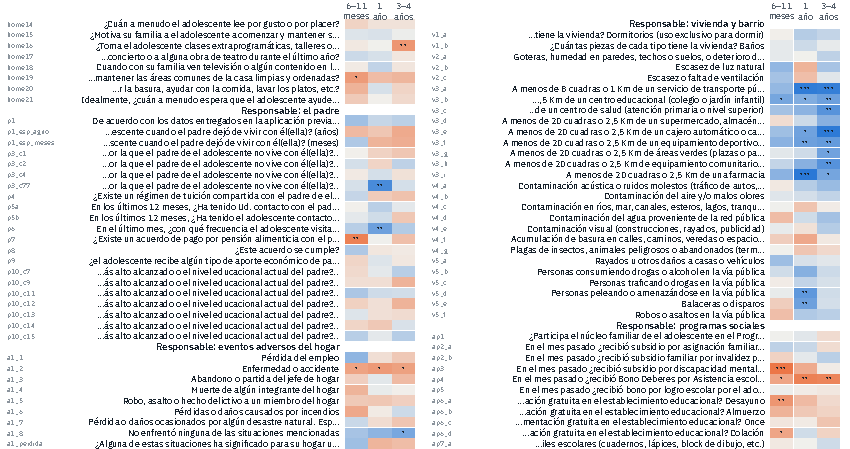
\includegraphics[height=0.83\textheight]{figuras/todo_2024_07.pdf}
\end{frame}
\begin{frame}
\frametitle{Todas las variables de 2024 (8/10)}
\centering
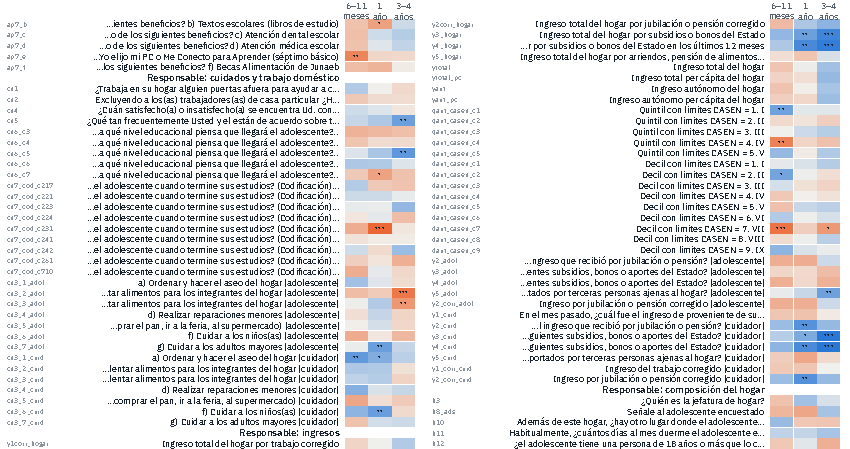
\includegraphics[height=0.83\textheight]{figuras/todo_2024_08.pdf}
\end{frame}
\begin{frame}
\frametitle{Todas las variables de 2024 (9/10)}
\centering
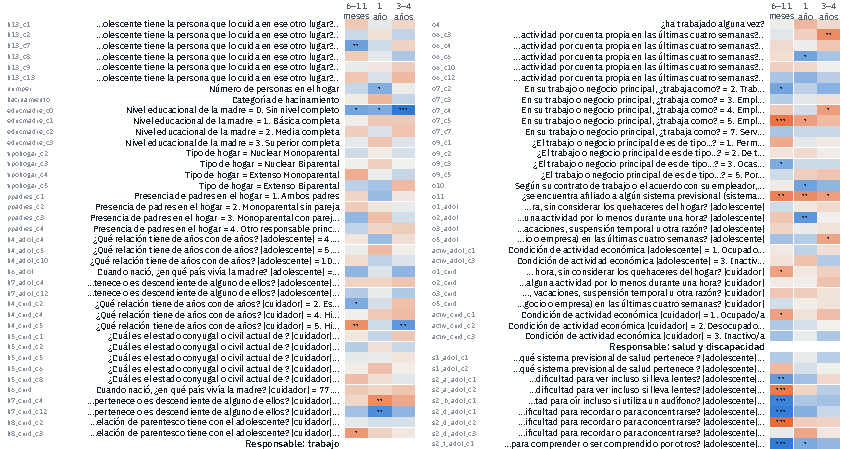
\includegraphics[height=0.83\textheight]{figuras/todo_2024_09.pdf}
\end{frame}
\begin{frame}
\frametitle{Todas las variables de 2024 (10/10)}
\centering
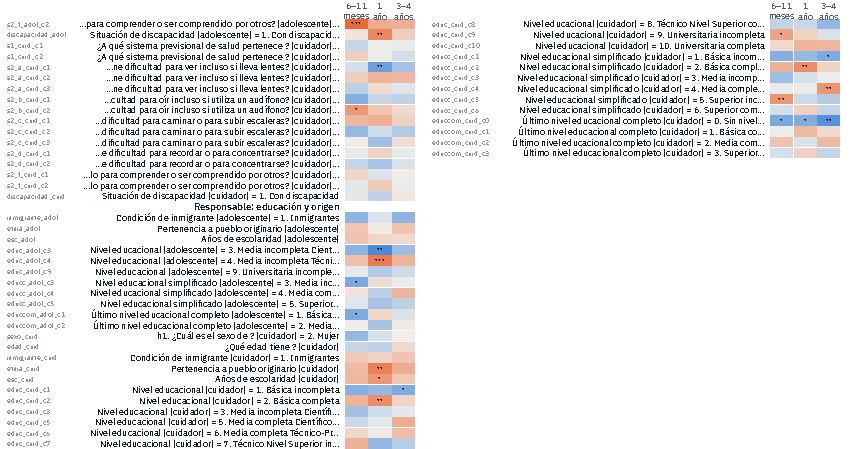
\includegraphics[height=0.83\textheight]{figuras/todo_2024_10.pdf}
\end{frame}

\end{document}
